The HPS experiment used a Silicon Vertex Tracker (SVT) and an electromagnetic calorimeter (ECal). The SVT, located inside of a dipole magnet, measures particle momenta and the interaction vertex position of the $e^+e^-$ pairs. The ECal triggers the readout of physics events and measures particle energy and time. \par
The HPS experiment is located in the downstream alcove of Hall B at Jefferson Lab. The Continuous Electron Beam Accelerator Facility (CEBAF) produces an electron beam which passes through Hall B to the alcove where the beam interacts with the HPS target housed inside the pair spectrometer magnet with the SVT. This interaction yields particle pairs and beam-scattered electrons which pass through the six layers of the SVT before depositing their energy in the ECal for event readout.

\section{Continuous Electron Beam Accelerator Facility}

The CEBAF accelerator at Jefferson Lab generates the electron beam used in the HPS experiment. CEBAF can deliver continuous electron beams to multiple experimental halls simultaneously. The CEBAF accelerator is a recirculating linac in the shape of a racetrack through which electron beam bunches can pass multiple times, boosted in energy with each pass, before being delivered to a specific hall. 

\begin{figure}[htb]
  \centering
      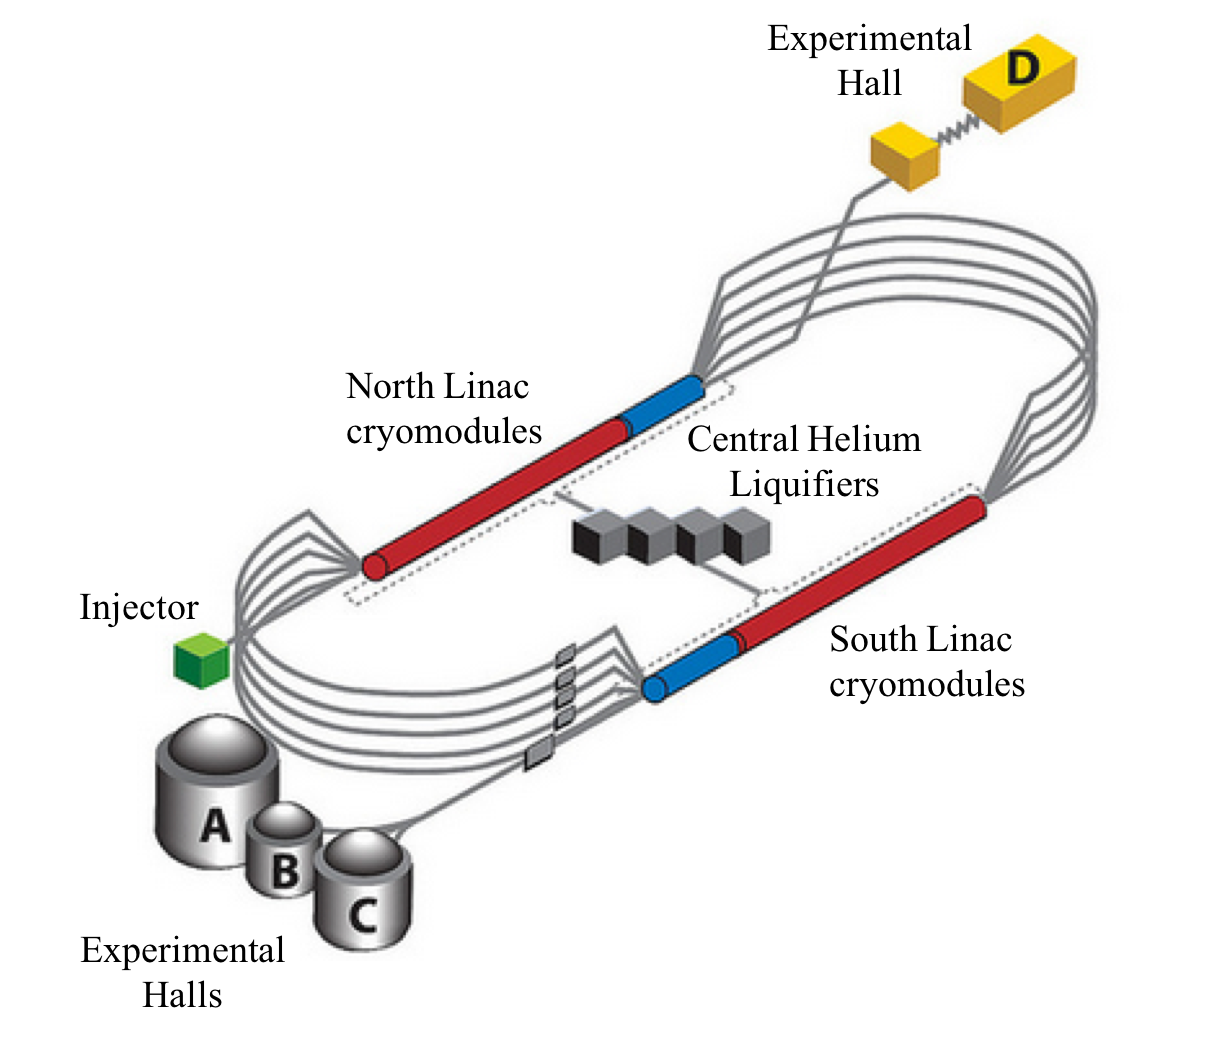
\includegraphics[width=0.75\textwidth]{pics/experiment/cebafLabel.png}
  \caption[CEBAF accelerator]{A drawing of the CEBAF accelerator. The electron beam is produced at the injector and can circulate through up to five passes around the race track design of the accelerator. There are four experimental halls that can receive beam and run experiments, simultaneously: A, B, C, and D. CEBAF was upgraded prior to the HPS experiment to include additional cryomodules, a second Central Helium Liquifier (CHL), and a fifth pass in order to produce higher energy.}
  \label{Figure:cebaf}
\end{figure}

CEBAF can provide continuous electron beams with energies up to 11~GeV and intensities up to approximately 100~$\mu$A to each of the four experimental halls. CEBAF was upgraded from producing 1.1~GeV per pass to 2.2~GeV per pass in 2014. 
%The injector energy is 100~MeV, designed for a maximum of five passes (upgraded from four passes) with %an energy per pass of 2.2~GeV (upgraded from 1.1~GeV). These upgrades double the maximum energy %output of the accelerator. While the accelerator frequency operates at 1500~MHz, a new 750~MHz RF %separator was installed in order to provide beam to all four halls simultaneously. With these upgrades, the %halls can receive the beam at 250 or 500~MHz and operate at different energies \cite{Kazimi_2013}. 

HPS was the first experiment to run in Hall B after the accelerator was upgraded. After a problem occurred in one central helium liquifier (CHL) during the engineering run in the spring of 2015, HPS obtained dedicated beam time as one of the few experiments that could continue to take physics data with the accelerator operating at a single pass using the remaining CHL. The resulting energy for the 2015 engineering run, 1.05~GeV, would have been impossible to obtain with the simultaneous running of other experiments requiring 2.2~GeV per pass.  

\section{Beamline}
The HPS experiment is installed in the downstream alcove of experimental Hall B at Jefferson Lab as shown in Figure~\ref{Figure:hallB}~\cite{beamline_nim_2017}. Due to the construction of the CLAS12 detector in Hall B as part of the CEBAF upgrade, HPS running was planned for nights and weekends when running beam would not interfere with CLAS12 construction. After the partial failure of the CHL, HPS received dedicated, continuous running during May of 2015 in support of the engineering run. 

\begin{figure}[htb]
  \centering
      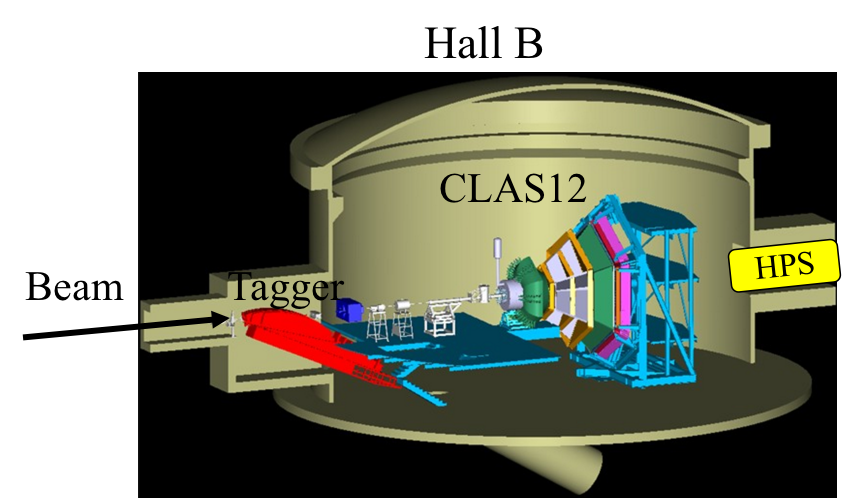
\includegraphics[width=0.6\textwidth]{pics/experiment/hallB.png}
  \caption[HPS location in Hall B]{The HPS experiment is in the downstream alcove of Hall B and ran while not interfering with CLAS12 construction.}
  \label{Figure:hallB}
\end{figure}

\begin{figure}[htb]
  \centering
      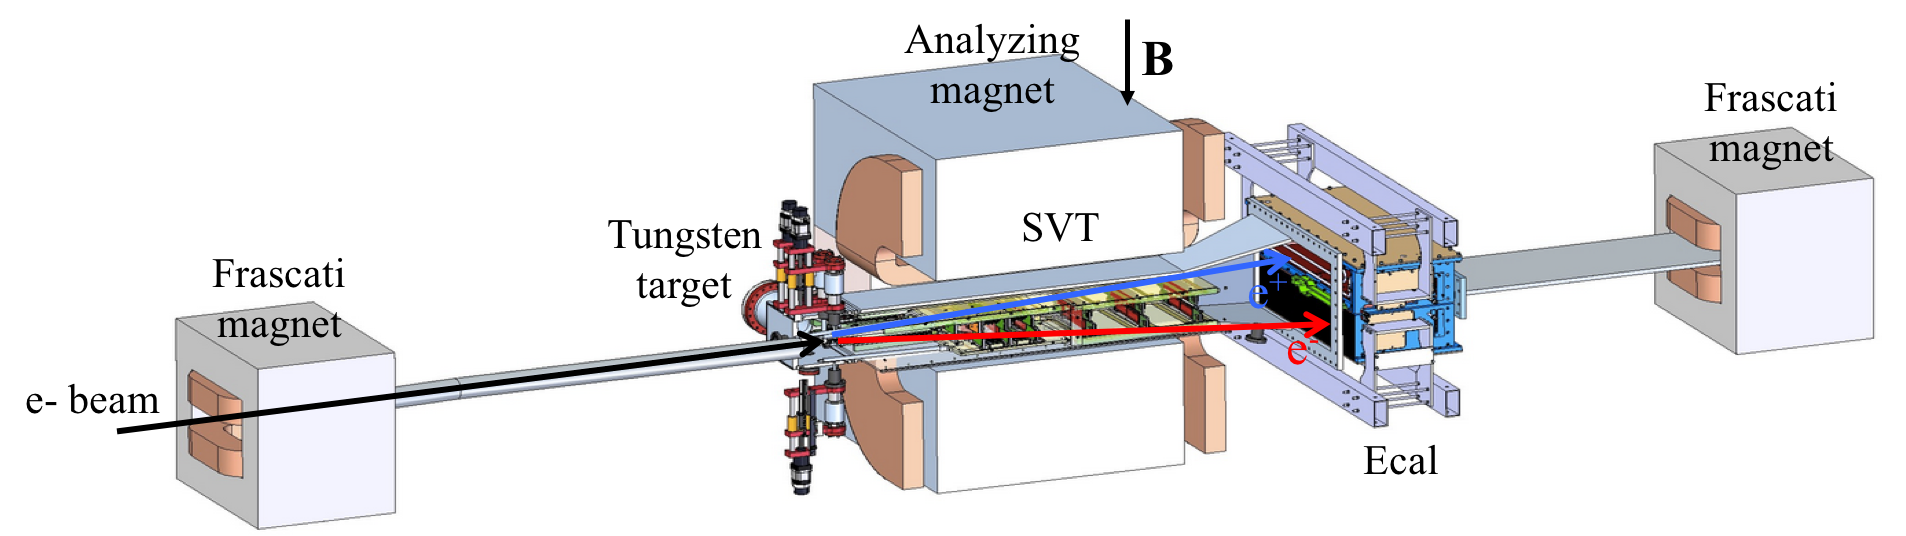
\includegraphics[width=1.0\textwidth]{pics/experiment/hpsBeamline.png}
  \caption[HPS beamline]{A drawing of the HPS experiment. After the electron beam passes through Hall B and into the alcove, the beam enters the first Frascati magnet. The electron beam hits the tungsten target, located in the Spectrometer magnet, at an angle of approximately 30.5~mrad. Particles created from the interaction of the beam at the target pass through the six tracking layers of the SVT before depositing their energy into the ECal.}
  \label{Figure:hpsBeamline}
\end{figure}

\begin{figure}[htb]
  \centering
      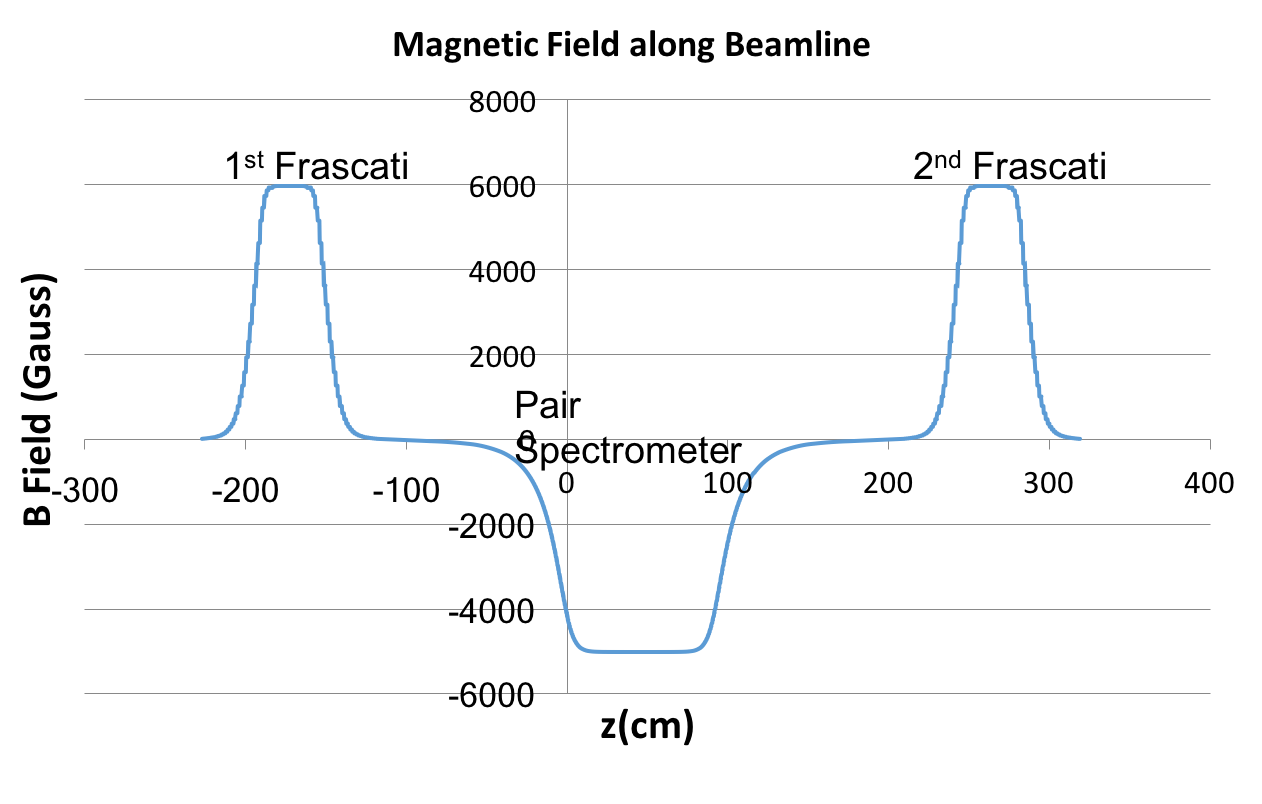
\includegraphics[width=1.0\textwidth]{pics/experiment/bfield.png}
  \caption[HPS magnetic fields]{The dipole magnetic field values for 2.2~GeV running where $z$ is the distance along the beamline from the target.}
  \label{Figure:bField}
\end{figure}

\begin{figure}[htb]
  \centering
      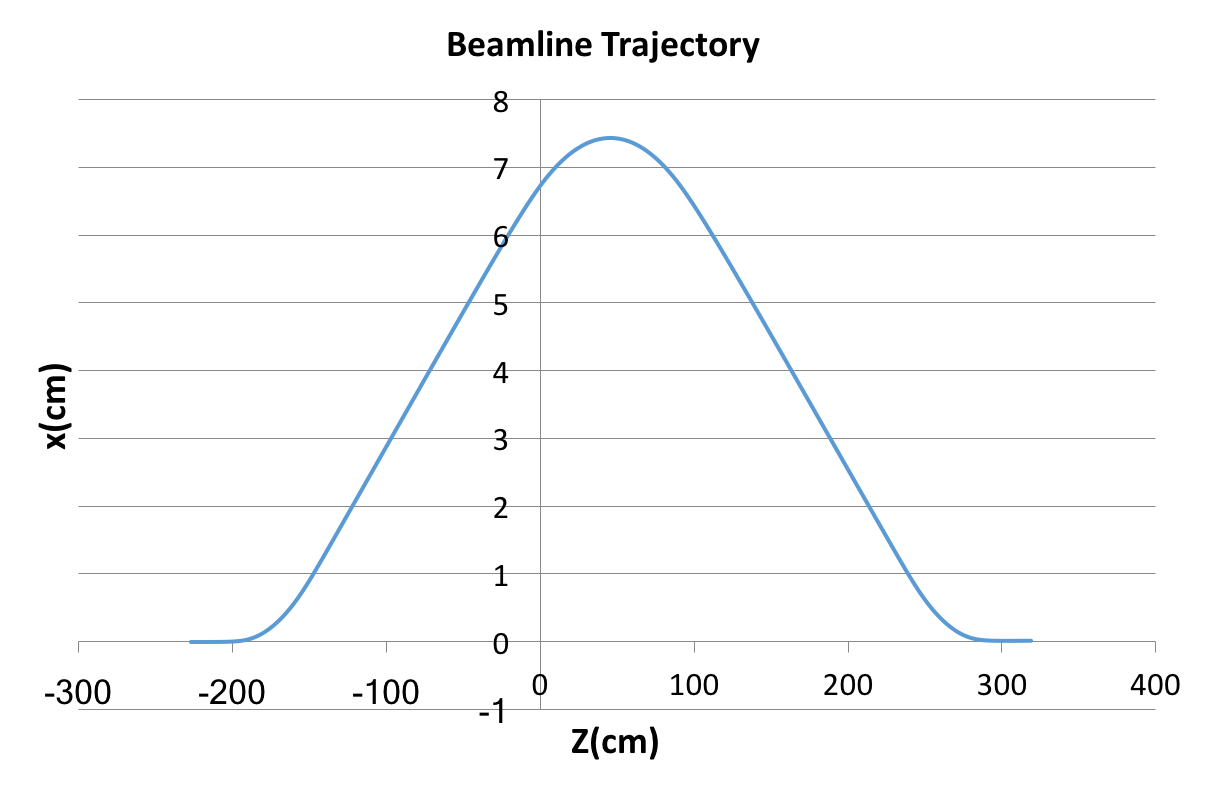
\includegraphics[width=1.0\textwidth]{pics/experiment/feetrajectory.png}
  \caption[Charged particle trajectory in HPS beamline]{The horizontal trajectory of a 2.2~GeV electron through the three dipole chicane along the beamline where $z$ is the distance along the beamline and $x$ is transverse to $z$. The target position is at $z=0$.}
  \label{Figure:trajectory}
\end{figure}

\begin{figure}[htb]
  \centering
      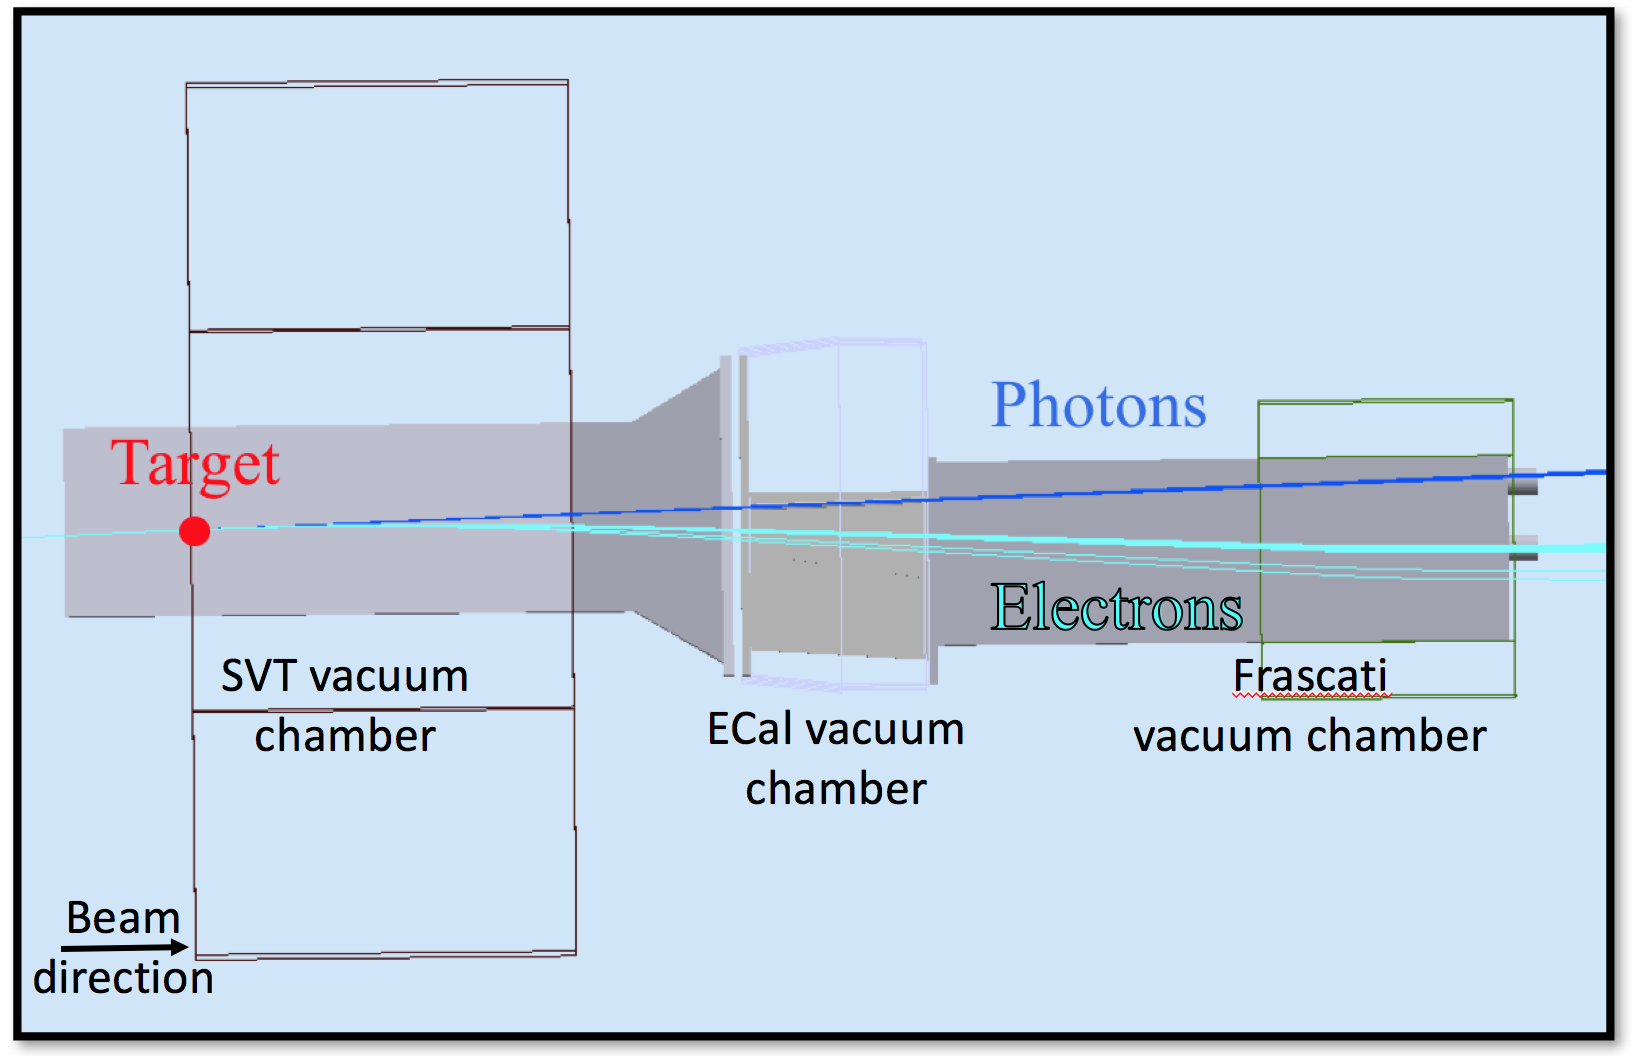
\includegraphics[width=0.8\textwidth]{pics/experiment/hpsbeam_v2.png}
  \caption[HPS beamline simulation in GEMC]{A bird's eye view of the HPS beam line shows the straight line trajectory of the photons from the HPS target through the SVT, ECal, and last vacuum chamber. The trajectory of the beam electrons in the magnetic field can be seen as passing through the cut outs in the vacuum chambers in order to pass through to the beam dump. The photons also have a clear, straight-line trajectory through the HPS vacuum chambers.}
  \label{Figure:gemc}
\end{figure}

%\begin{figure}[htb]
%  \centering
%      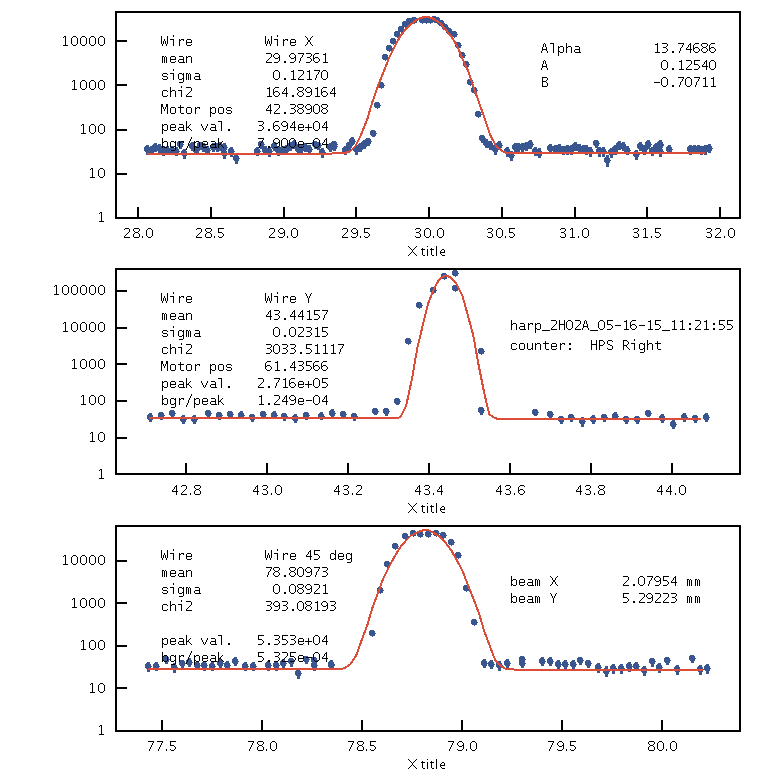
\includegraphics[width=0.75\textwidth]{pics/experiment/harpScan.png}
%  \caption[Beam profile from harp scan during 2015 run]{Harp scan showing the beam profile during May 2015 running. This particular harp scan is in the Hall B logbook, entry 3341231. The beam line profile in this scan is 122$\mu$m wide in $x$ by 23$\mu$m in $y$.}
%  \label{Figure:harpScan}
%\end{figure}

\begin{figure}[hbt]
%\begin{center}
\begin{minipage}{0.65\textwidth}
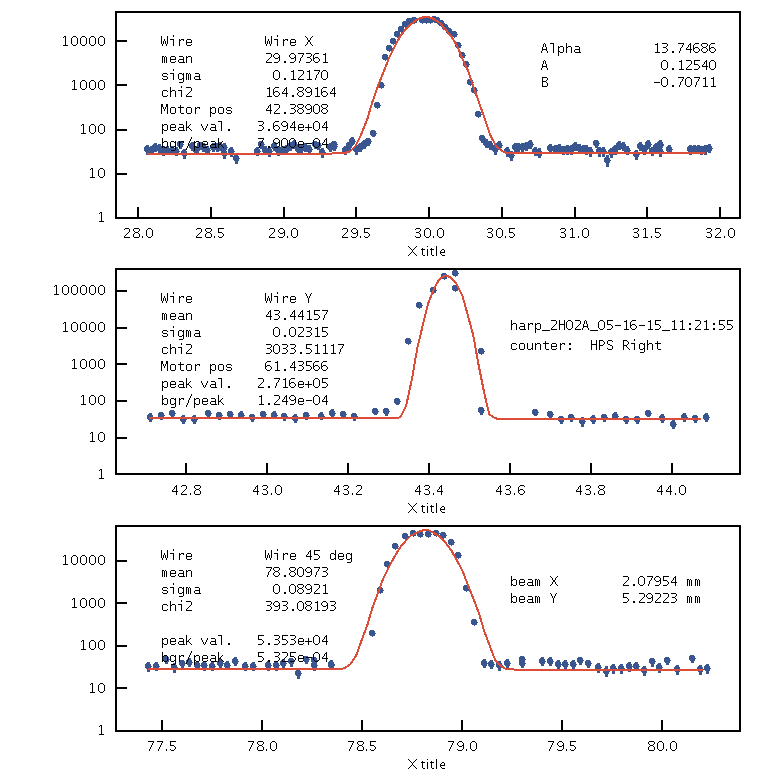
\includegraphics[width=\textwidth]{pics/experiment/harpScan.png}
%\end{center}
\end{minipage}\hfill\begin{minipage}{0.32\textwidth}
\caption[Beam profile from harp scan during 2015 run]{ \label{fig:harpScan} \baselineskip 11pt
Harp scan showing the beam profile during May 2015 running. This particular harp scan is in the Hall B logbook, entry 3341231. The beam line profile in this scan is 122~$\mu$m wide in $x$ by 23~$\mu$m in $y$.}
\end{minipage}
\end{figure}


The tagger magnet as depicted in Figure~\ref{Figure:hallB} was used for initial beam tuning from the accelerator before sending the beam through to the HPS detectors. By energizing the tagger magnet, the electron beam was visible at the tagger dump viewer and could be aligned at the center of the viewer. Before sending the beam to HPS, harp scans were performed to measure the position and width of the beam spot~\cite{beamline_nim_2017}. Once the harp scans showed the beam to be of an acceptable size and position upstream of HPS, the tagger magnet was de-gaussed for HPS running. Without the tagger magnet on, the electron beam passes through the hall to the HPS setup as shown in Figure~\ref{Figure:hpsBeamline}. \\
\indent The HPS setup consists of a three-dipole chicane with magnetic fields in the vertical direction. The target and the SVT are housed in the central magnet known as the spectrometer, or analyzing magnet. The magnet has a pole length of 91.44~cm and width of 45.72~cm. For 2.2~GeV electrons, the central magnetic field of the spectrometer magnet is 0.5~T~\cite{beamline_nim_2017}. For other beam energies, the analyzing magnet magnetic field is scaled accordingly. In the engineering run in May 2015, with a beam energy of 1.056~GeV, the spectrometer had a central field value of 0.24~T. The ``Frascati" magnets, one on each side of the analyzing magnet, have magnetic fields opposite to that of the analyzing magnet such that the integrated field value over the length of the pole value of each Frascati is half of the integrated field value of the analyzing magnet. This ensures that the beam will end at the same location whether the chicane is energized or not and that the trajectory of beam energy electrons in the magnetic field is consistent across different beam energies. The magnetic field of the HPS beam line in the chicane is shown in Figure~\ref{Figure:bField}.\\
\indent The magnetic fields of the magnets were carefully measured and mapped. The trajectory of particles was studied using these magnetic field maps that included fringe field effects. The position of the spectrometer magnet with respect to the Frascati magnets was optimized from these field mappings. The horizontal trajectory of a beam energy electron is shown in Figure~\ref{Figure:trajectory}.\\
\indent In Figure~\ref{Figure:trajectory}, the target position is where at $z=0$. The entry angle of the beam at the target was determined to be approximately 30.5~mrad. At 70~cm from the target, the spectrometer magnet and vacuum chamber are centered on the position of the photon trajectory from the target such that the photons pass unobstructed through all subsequent vacuum chambers. The pair spectrometer magnet was placed 8.87~cm beam left, thus placing the HPS target position 2.14~cm to the right of the magnet center line. By modeling the vacuum chambers and magnetic fields in the GEant4 Monte Carlo (GEMC) framework, the particle trajectories through the HPS beam line can be observed as in Figure~\ref{Figure:gemc}.\\
\indent As shown in Figure~\ref{Figure:gemc}, the beam energy electrons pass through the exit hole of the last vacuum chamber (contained in the second Frascati dipole) and continue traveling to the Faraday cup where the beam charge can be measured. The beam line was modeled in GEMC and, in real running, utilized a multitude of monitors to ensure clear passage of the beam.\\
\indent The passage of the beam through the HPS beam line was monitored using beam position monitors (BPMs), wire scans with halo counters, beam viewers, and a Faraday cup. The three upstream nA BPMs gave continuous beam current and position readings. These BPMs can indicate that the beam is scraping the beam pipe when the current readings fluctuate and differ with respect to each other. The current readings from the BPMs were compared to the current reading at the Faraday Cup (located downstream of the HPS beam line at the dump). When the beam current is at 50~nA or below, the reading at the Faraday Cup current is roughly the same as the current read out by the upstream BPMs and indicates no beam scraping in the beam pipe. When operating at currents above 50~nA, it was standard to insert a beam blocker in front of the Faraday Cup in order to protect it. The beam stopper would then create an offset in the Faraday Cup current readout and the actual beam current. Additionally, a fluorescent viewer screen at the Faraday Cup was used to show the beam position.  A video camera streaming a view of the screen was used for remotely observing the relative beam position on the screen. \\ 
\indent The wire harp scans measured the beam position through beam-wire interactions (as compared to the passive, continuous readout employed through the BPMs). A harp scan moves strong wires through the beam vertically, horizontally, and diagonally while  downstream halo counters measure the scattered beam electron spray. The halo counters are photomultiplier tubes (PMT) strapped around the beam pipe line. The intensity of the electron spray detected by the PMTs is proportional to the beam charge interacting with the wire. A typical harp scan from the 2015 run is shown in Figure~\ref{fig:harpScan}.\\
\indent The beam profile is narrower in $y$ (vertically) than in $x$ (horizontally). The proposed beam profile for the HPS experiment was 50~$\mu$m in $y$ and 300~$\mu$m in $x$ in order to allow for precise vertex reconstruction. Most of the 2015 running had a beam profile of no larger than 50~$\mu$m in $y$ and 150~$\mu$m in $x$. 

\subsection{Beam line protection}
The SVT is ideally as close to the beam as possible in order to maximize acceptance for heavy photons. The nominal SVT position has the first layer of the SVT at $\pm0.5$~mm from the active beam. Passive and active measures were employed during experimental running to prevent damage to the silicon if the beam position or quality changed during running. A collimator, a 1~cm thick tungsten plate with a slit through which the beam can pass, was placed upstream of the SVT. A collimator prevents direct damage to the silicon should the beam move vertically from its nominal position by diffusing the beam. For the 2015 run, the 4~mm slit width was used. \\
\indent The active beam line protection element is the Fast Shut Down (FSD) system. The FSD, when triggered, can shut off the electron beam in 1~ms. HPS used the halo counters closest to the HPS experiment to trigger the FSD when the beam shifted or the quality significantly deteriorated. When the beam shifted vertically, it would first hit the inactive region of the SVT sensors and scatter, increasing the rates in the halo counters. When the rates surpassed a pre-determined threshold, the FSD was tripped. If the beam hit the collimator, this also increased the rates in the halo counters and tripped the FSD. 

\subsection{Target}

The primary HPS target is a thin tungsten foil that is mounted on a support frame that can be fully retracted from the beam when not in use. For 1.1~GeV and 2.2~GeV running, the design thickness of the target tungsten foil is 0.125$\%$ radiation lengths (approximately 4~$\mu$m). The measured thickness of the actual target was 0.116$\%$. There is also a tungsten target of 0.25$\%$ radiation lengths for future running at 4.4~GeV and 6.6~GeV. The target support frame inserts the foil target from above the beam using a stepping motor linear actuator. The bottom of the target foil is frame-less so that the target can be inserted into the active beam without interruption.   

\section{Silicon Vertex Tracker}
\begin{figure}[htb]
  \centering
      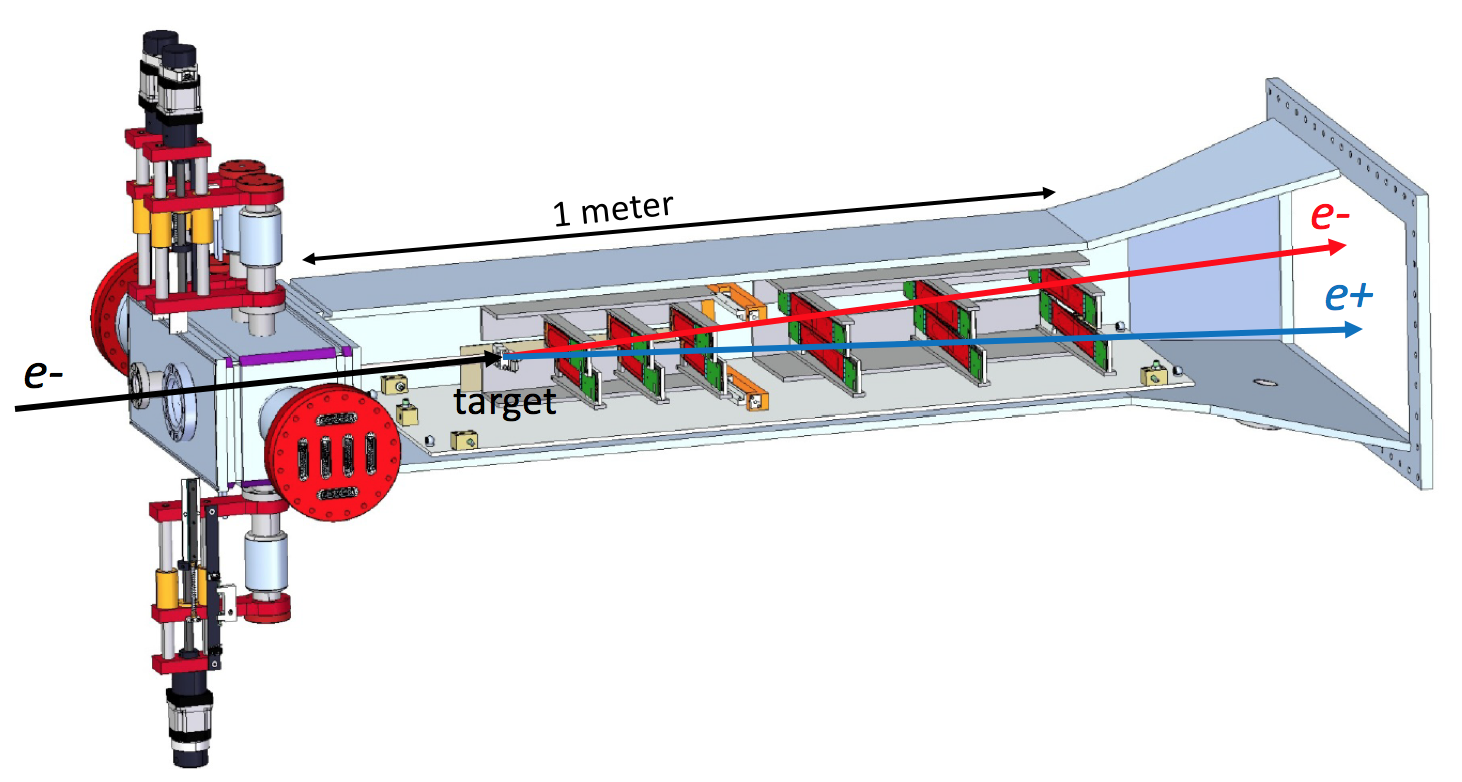
\includegraphics[width=1.0\textwidth]{pics/experiment/svt.png}
  \caption[Rendering of the HPS SVT]{A rendering of the HPS SVT. The beam enters from the left through the vacuum box. The silicon sensors are shown in red, and the hybrid readout boards are shown in green.}
  \label{Figure:svt}
\end{figure}

\begin{figure}[h]
  \centering
      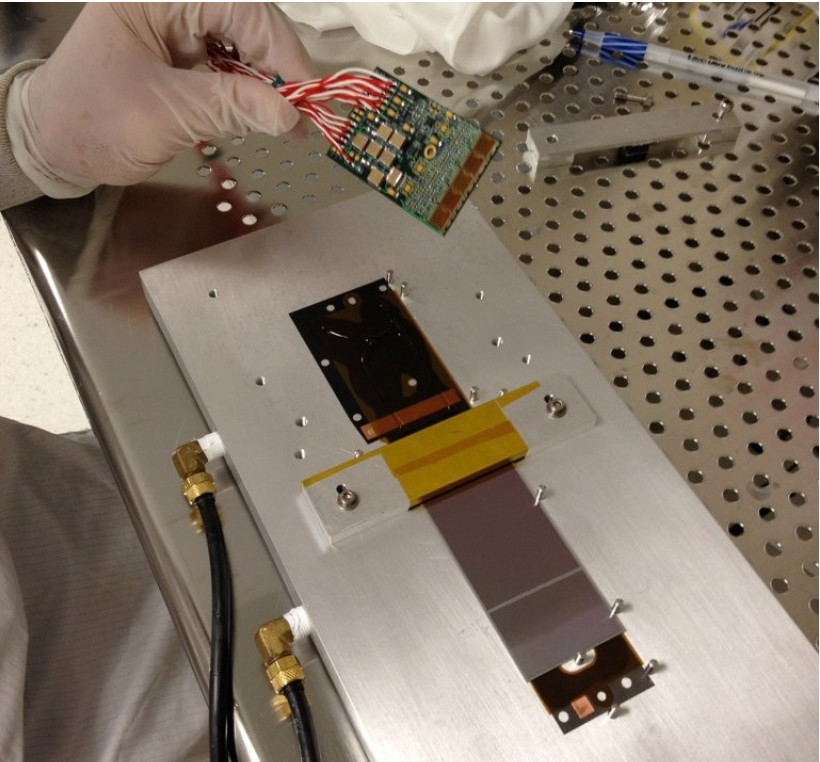
\includegraphics[width=0.5\textwidth]{pics/experiment/svtSensorAssembly.png}
  \caption[Assembly of a half module of the SVT ]{A half module is being assembled for Layers 1-3 of the SVT. A readout hybrid with the APV25 chips is being attached to the frame along the silicon sensor.~\cite{collaboration_heavy_2013}}
  \label{Figure:svtAssembly}
\end{figure}

The Silicon Vertex Tracker (SVT) measures particle momentum and trajectories through a magnetic field in order to reconstruct the invariant mass and the vertex position of the $e^+e^-$ pair. The SVT is composed of six layers of 0.7$\%$ radiation length-thick silicon placed downstream of the target and housed in a vacuum chamber within the analyzing magnet. The SVT is separated into top and bottom halves that can be positioned vertically above and below the beam. Nominally, the SVT operates with a 15~mrad opening angle such that the first layer of the SVT is at $\pm$0.5~mm from the active beam. A drawing of the SVT is shown in Figure~\ref{Figure:svt}.

The SVT is located in a magnetic field such that particles are bent horizontally (field points downward). Each of the six layers is composed of two silicon strip detectors capable of measuring a hit position in one dimension. By setting the strips at a stereo angle with respect to one another, each layer of the SVT is capable of three-dimensional hit reconstruction. The first three layers of the SVT are one silicon strip sensor-wide and have a stereo angle of 100~mrad between the strips. The last three layers of the SVT are two strip sensors-wide in order to better match the ECal acceptance. The stereo angle between the sensors in layers four through six is 50~mrad. The axial sensors are oriented horizonally whereas the stereo sensors are angled with the lower end closer to the beam plane on the positron side (beam left) where the background is less intense. The different stereo angles are used to eliminate ghost hits that can generate ghost tracks. The first five layers of the SVT cover the ECal acceptance while the sixth layer has a slightly reduced acceptance but can be used to improve track reconstruction. The full track reconstruction only requires five hits per track in order to pick up tracks that may be missing hits due to an inefficiency. \\
\indent The hybrid readout boards on each sensor house the APV25 readout chips that connect the sensor to the data acquisition (DAQ) system. The power to the APV25 chips is supplied through the hybrid, and the temperature of the strip is actively monitored at the hybrid. The heat generated by the operating hybrid  flows through the aluminum support structure. As the sensors are cooled for operation, the support structure and sensor contract at slightly different rates. In order to maintain the sensor at a constant tension, one end of the sensor is attached to a spring pivot. The assembly of a silicon sensor is shown in Figure~\ref{Figure:svtAssembly}.

The APV25 samples the signals on the strips every 24~ns and stores the results in a pipeline. Once a trigger is received, the pipelines are read out. The readout yields six samples at 24~ns intervals that can be fit to reconstruct the waveform. A 4-pole functional fit was used to extract the time and amplitude of the corresponding hit. A latency time that is configured in the SVT DAQ is used to correctly determine which channel pipelines are read out that correspond to the trigger. The latency time is approximately equal to the time delay of the trigger. Some early data in the 2015 engineering run was lost due to incorrect latency timing. 


\section{Electromagnetic Calorimeter}
The ECal was used to trigger events and measure particle energy and timing. The ECal is a homogeneous calorimeter comprised of 442 trapezoidal PbWO$_4$ scintillating crystals, each read out by a large area avalanche photodiode (APD) attached to the back of each crystal~\cite{Balossino201789}. The crystals are re-purposed from the former CLAS IC detector and have been upgraded with larger avalanche photodiodes. Each crystal is trapezoidal in shape and 16~cm long with the front and back faces measuring 1.3$\times$1.3~mm$^2$ and 1.6$\times$1.6~mm$^2$, respectively. The calorimeter layout is shown in Figure~\ref{Figure:ecalface}. 

\begin{figure}[h]
  \centering
      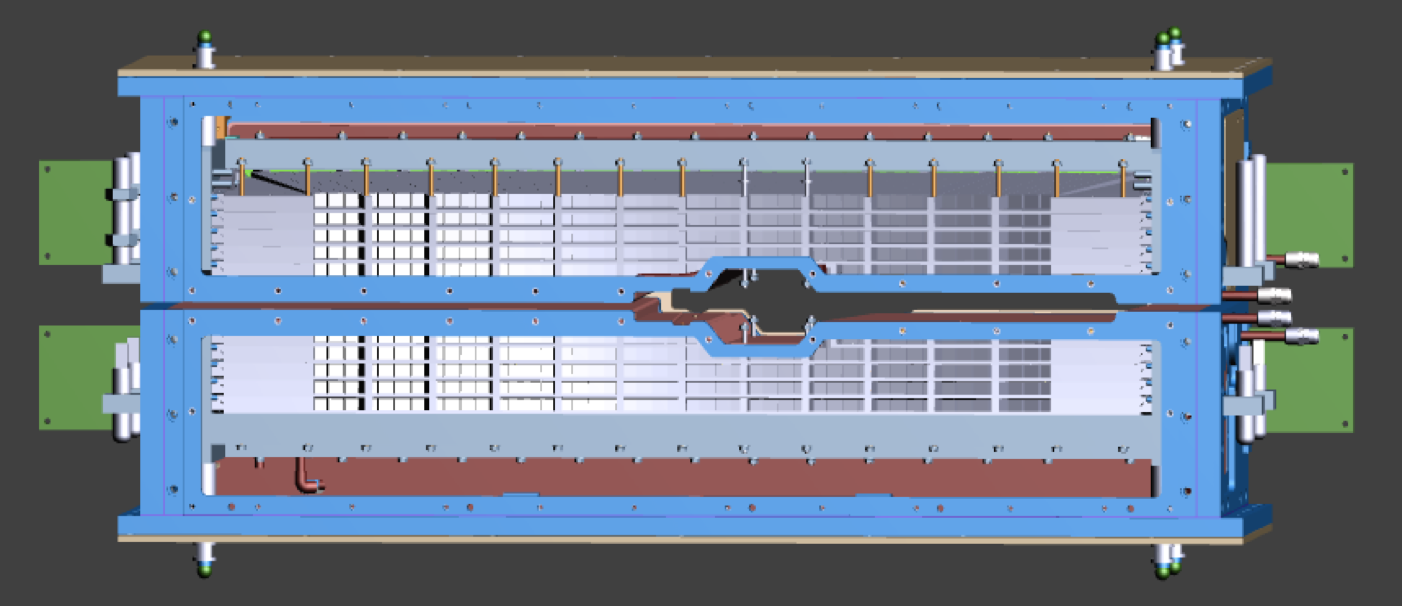
\includegraphics[width=0.85\textwidth]{pics/experiment/ecalface.png}
  \caption[Drawing of the ECal assembly face]{Drawing of the ECal assembly face, looking downstream along the beam direction. The ECal is assembled in two vertical halves and has a gap between allowing for the electron and photon beams. Beam electrons resulting from energy losses in the target are deflected in the dipole field toward the beam right and result in the ``sheet of flame". The ECal includes a cut out in order to avoid the high rates that result from detecting these particles.}
  \label{Figure:ecalface}
\end{figure}

\begin{figure}[h]
  \centering
      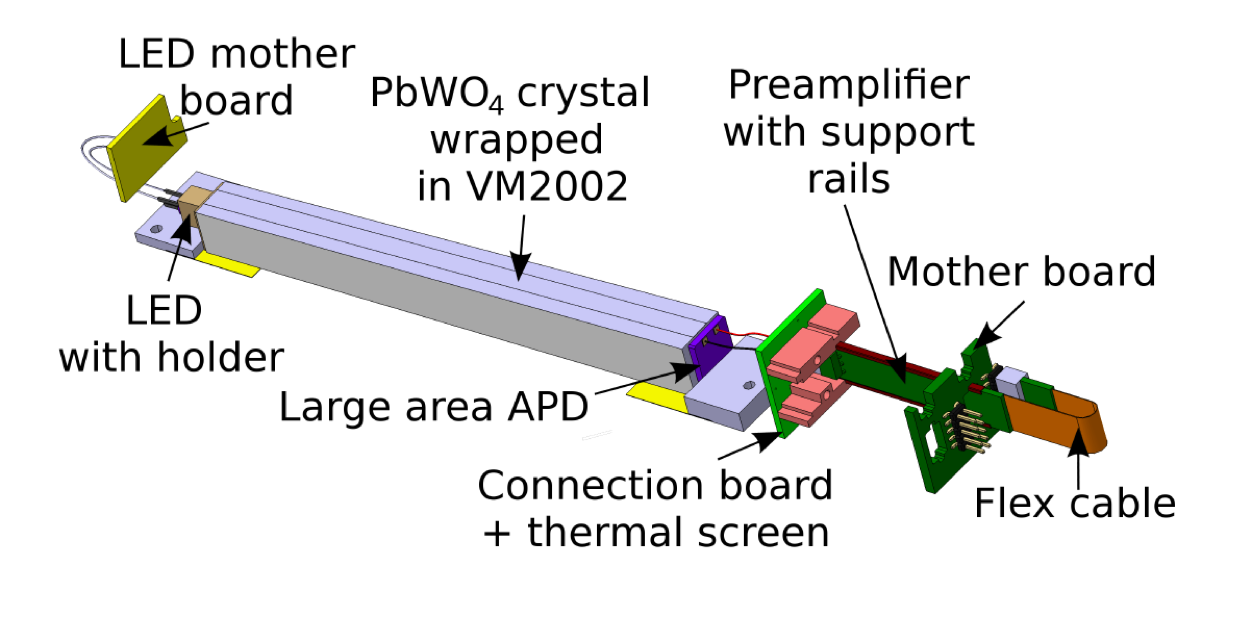
\includegraphics[width=0.85\textwidth]{pics/experiment/crystal.png}
  \caption[Single ECal module]{Drawing of an ECal crystal in readout configuration. An LED is placed at the front of each crystal at the upstream end. Light is collected at the downstream face of the crystal with the APD. Electronic signals are amplified through the preamplifier. Power to preamplifiers and the APDs is supplied through the motherboard.}
  \label{Figure:crystal}
\end{figure}

\begin{figure}[h]
  \centering
      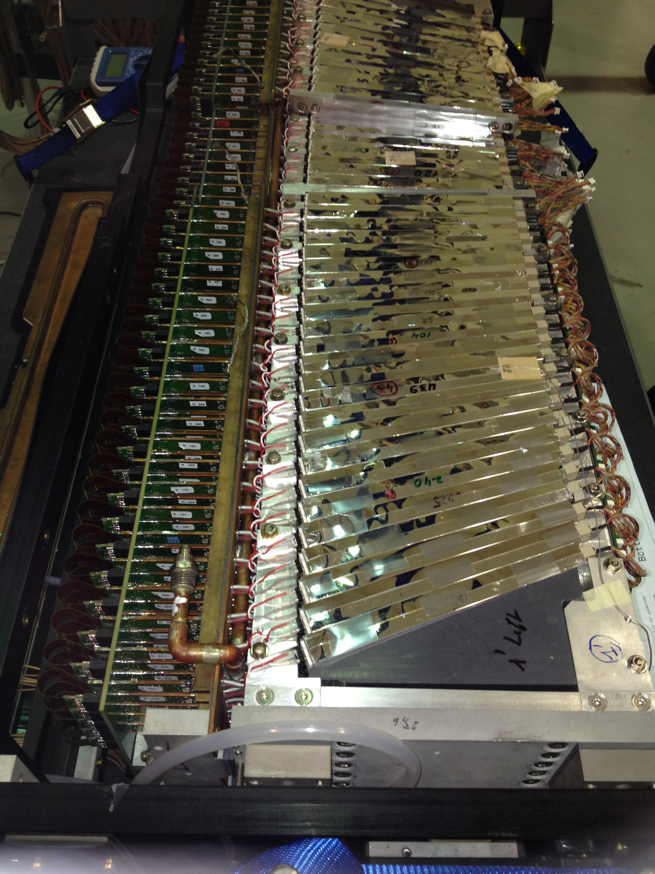
\includegraphics[width=0.5\textwidth]{pics/experiment/ecalAssembly1.png}
  \caption[Photograph of ECal crystals during assembly]{Photograph taken during assembly of the ECal from above. The preamplifiers attached to each crystal are shown on the left. As single layer of wrapped crystals are shown in their tray, and the LEDs attached to each crystal are shown on the right.}
  \label{Figure:ecalAssembly1}
\end{figure}

Each crystal is wrapped in a VM2002 reflecting foil in order to increase light collection. The original APDs used by the the IC had a surface area of 5$\times$5~mm$^2$, but these were upgraded for HPS running by replacing each original APD with a large area APD (model S8664-1010) of surface area 10$\times$10~mm$^2$. The upgraded APDs collect four times more light than the old APDs. The larger signals require less electronic amplification of the signal and improve the signal-to-noise ratio. This allows a lower energy threshold for module readout and improves the energy resolution. \\
\indent The ECal is constructed as two separate vertical halves in order to avoid the 15~mrad vertical zone of excessive electromagnetic background along the beam line. The crystals in each half are arranged in five layers of 46 crystals. The layer of crystals closest to the beam in each half has nine crystals removed to allow for the passing of the unscattered electron beam. The two halves of the ECal are each at 2~cm from the  horizontal electron beam plane.\\
\indent As a particle enters the ECal, it initiates an electromagnetic shower by either bremsstrahlung or pair production. The secondary particles then produce more particles through bremsstrahlung and photon pair production giving rise to a cascade of particles, decreasing in energy. After the electron energy is too low to yield further particles, the remaining energy is deposited through ionization and excitation. The resulting scintillation photons hit the APD that converts the collected photons into an electronic signal via the photoelectric effect. Each APD is attached by a twisted pair connector to a preamplifier which converts the signal current to voltage and has low input impedence and noise.  

The gain of the APDs and the scintillation of the crystals in the ECal are temperature-dependent. An Anova A-40 external chiller operating at 17$\degree$C pumps cool water through copper cooling pipes that run along the inside of the ECal at the top, bottom, front, and back faces of the structure. The internal temperature of the ECal was monitored using sixteen thermocouples located at various locations within the ECal. The thermocouples are read out using Omega D5000 series transmitters. Both devices are connected through RS-232 serial communications for external monitoring and alarms should the temperature change significantly.\\
\indent Low voltage power is supplied to the preamplifiers via an Agilent 6221 power supply operating at 5~V and approximately 4.1~A when all preamplifiers are connected. The high voltage to each of the 52 APD groups is supplied by CAEN A1520P modules in a SY4527 mainframe. Both voltage supplies are monitored and accessible for remote operations.  

\subsection{Light Monitoring System}
The Light Monitoring System (LMS) is a remotely-controlled upgrade to the ECal consisting of a bi-color LED attached to the front of each ECal module. PbWO$_4$ scintillating crystals are relatively radiation tolerant but have a known decrease in light yield after exposure to enough radiation~\cite{Batarin2005543}. This effect is non-uniform in the ECal as different modules are exposed to different levels of radiation. The LMS can turn individual modules on and off independently. This proved useful in checking each channel's functionality and correct cabling. The LEDs were selected such that the shape and duration of the emitted flash generates a pulse shape similar to the scintillation effect in the PbWO$_4$crystal~\cite{battaglieri_ft_clas12}.\\
\indent Each crystal has a plastic LED holder glued to the front that contains a bi-color LED, model RAPID 56-0352, capable of emitting red and blue light. The use of two different colors allows for the study of different effects in the ECal modules. The blue LED has a wavelength close to the 430~nm emission peak of PbWO$_4$  \cite{battaglieri_ft_clas12} and is used to check for radiation damage in the crystal as this spectrum would be most affected. The red light is not sensitive to the radiation effects in the crystals, but is useful for checking the stability of the  APD gain.\\ 
\indent The LMS uses four driver boards on each half of the ECal. The four driver boards on each half are connected to one of two main controllers, and each driver can turn on a single LED at a time. The controllers communicate with the LMS through ethernet and USB interfaces. The controller board for the top half of the ECal also contains the master clock signal that sets the rate at which the LEDs flash. This clock signal is sent to the bottom controller so that the driver boards on the bottom half of the ECal can flash at the same rate, and the clock signal is used to trigger LED events when the DAQ is used.\\
\indent During the initial assembly of the ECal, the LEDs were used to study the cross talk between ECal modules. The cross talk between channels was found to be 2$\pm$1$\%$ and generally occurred in modules of the same row to the immediate left and right of the triggered module. The effect most likely appears due to light leakage out the back face of the crystal where the APD does not cover the entire surface. The raw waveform response from a red LED signal in a single ECal module is shown in Figure~\ref{Figure:redSignal}. The units are given in mV which are a factor of four times less than the units of FADC.

\begin{figure}[htb]
  \centering
      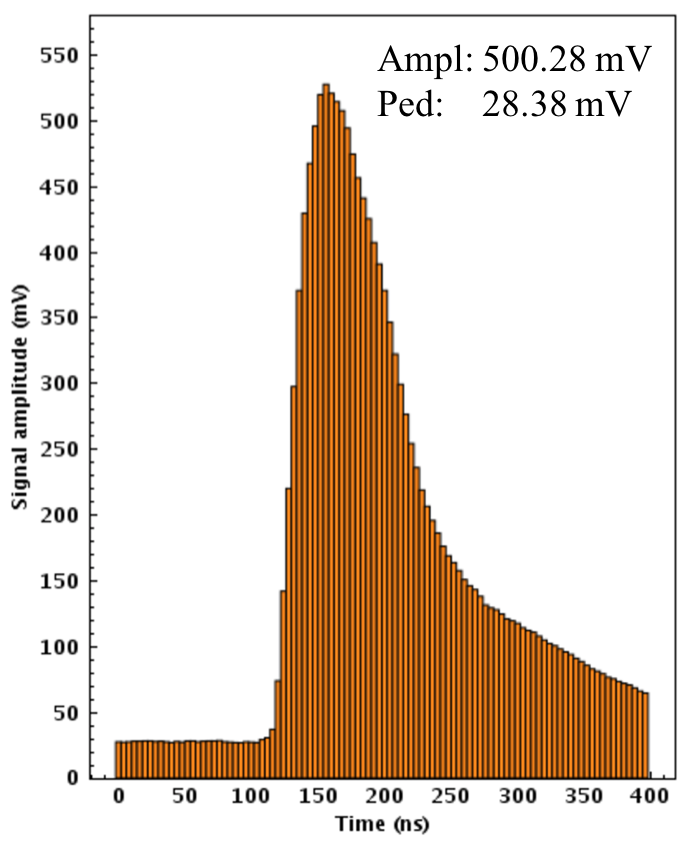
\includegraphics[width=0.5\textwidth]{pics/experiment/ledSignal.png}
  \caption[LED signal in ECal FADC]{A red LED in a single ECal module as readout through the FADC (see section~\ref{pulsefitting})}
  \label{Figure:redSignal}
\end{figure}
Before and after periods of long beam run times, the ECal gains were checked with the LEDs. The LED test ran a sequence of red and blue LED flashes so that the characteristic response of each module was measured. The typical results from an LED test are shown in Figure~\ref{Figure:redCompare}.

\begin{figure}[htb]
  \centering
      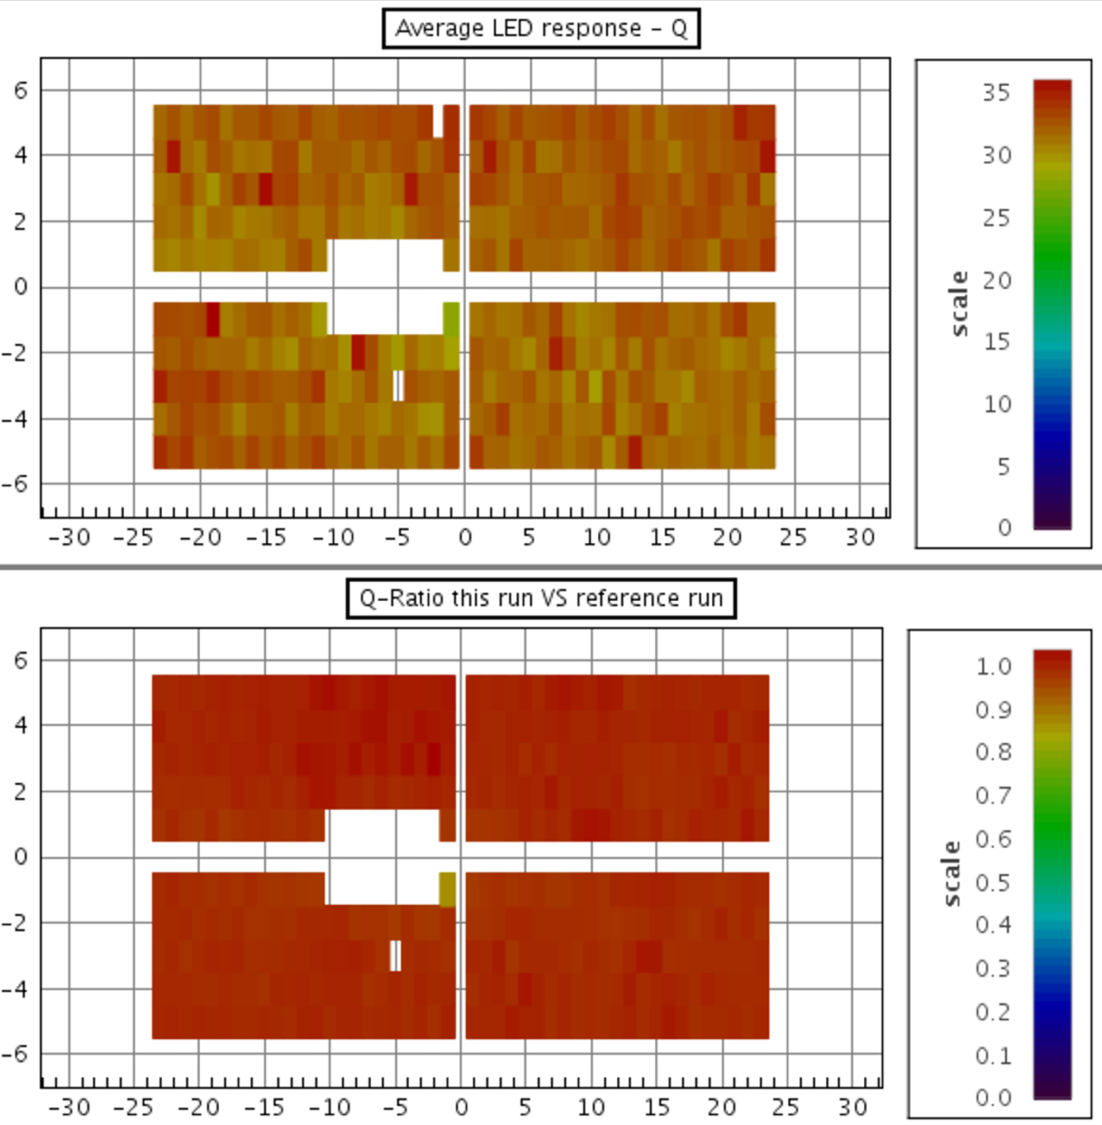
\includegraphics[width=0.65\textwidth]{pics/experiment/ledCompare.png}
  \caption[Results of a single LED run]{The top shows the LED response in each crystal for a specific LED run. The bottom compares each crystal with a its database value as stored from a previous LED run.}
  \label{Figure:redCompare}
\end{figure}
As shown in Figure~\ref{Figure:redCompare}, the individual ECal module response is given as the pulse-integral in units of GeV. The response values for individual crystals have large units of energy because the LED pulse is significantly longer than an actual scintillation pulse in the crystal. A LED test can show differences in the gain of individual crystals on the order of $1\%$ when compared to previous LED test results. During the 2015 engineering run, a 5$\%$ change in the gains across all modules occurred over the course of establishing production beam between February and April. This change was seen in LED response studies in addition to the gains obtained with cosmic energy calibration.

\subsection{Avalanche Photodiodes}


We upgraded the ECal by installing large area Hamamatsu S8664-3189 APDs for readout. APDs were used for reading out the ECal modules due to their ability to operate in the fringe magnetic field of the HPS beam line. Both the Institut de Physique Nucleaire d'Orsay (IPN) and Instituto Nazionale di Fisica Nucleare (INFN) groups in the HPS collaboration purchased the large area APDs for upgrade. As the IPN group re-designed the motherboards for the upgrade, INFN developed the testing apparatus so that the gain of each APD could be characterized and sorted into one of 52 high voltage groups to minimize response variations. The large area APDs are shown in Figure~\ref{Figure:apd}.

\begin{figure}[h]
  \centering
      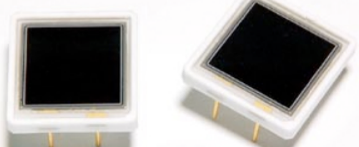
\includegraphics[width=0.4\textwidth]{pics/experiment/apd.png}
  \caption[Hamamatsu S8664-3189 large area APDs]{The Hamamatsu S8664-3189 large area APDs are $10\times10$~mm$^2$.}
  \label{Figure:apd}
\end{figure}

APDs are reverse-biased diodes with an internal high electric field that multiplies the electrons through an avalanche mechanism.  The characteristic gain of an APD depends on the temperature of the environment due to the interaction of the electrons with the phonons. The gain is inversely correlated with temperature.  The APD gains have a linear dependence on both voltage and temperature. Prior to grouping the APDs for installation in the ECal, each APD was tested and bench marked to check for quality and optimal operating voltage in order to achieve a pre-selected gain of 150. The testing apparatus was designed and installed by the group from INFN as the same procedure was used in the construction of the Forward Tagger~\cite{celentano_2014}. The apparatus is shown in Figure~\ref{Figure:apdtest}.

\begin{figure}[h]
  \centering
      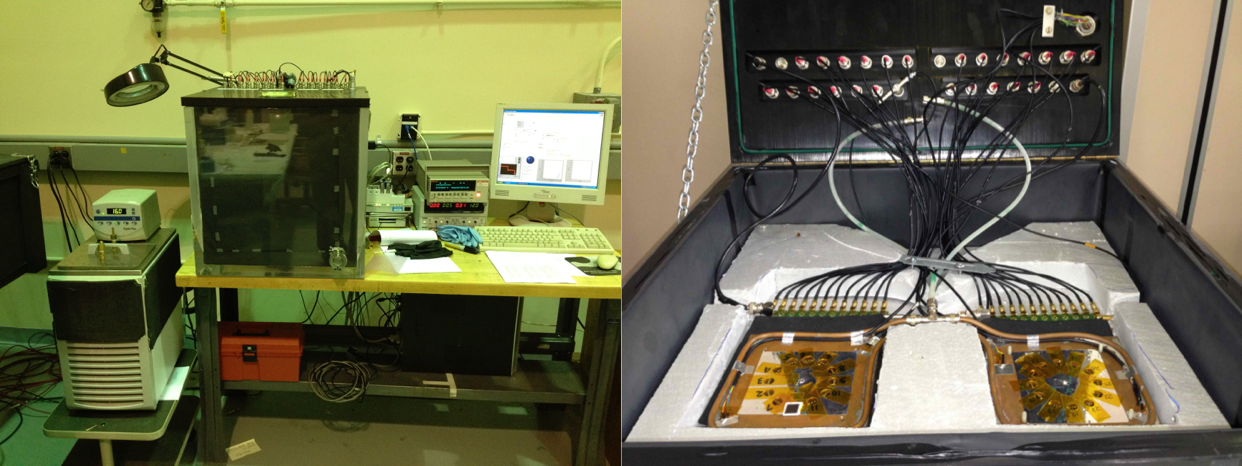
\includegraphics[width=0.7\textwidth]{pics/experiment/apdtests.png}
  \caption[Testing assembly for large area APDs]{On the left, the testing setup is shown and includes a chiller, the light-tight plastic box that contains the LEDs and APDs, an electrometer, and the data acquisition. On the right, the setup inside of the light-tight plastic box is shown that contains a copper cooling plate to maintain the chiller temperature, 10 slots on each side to hold APDs, and the LED in the center of each half.}
  \label{Figure:apdtest}
\end{figure}

In order to avoid condensation on the cooling lines, the temperature range for conducting the tests was limited to 16$\degree$C, 18$\degree$C, and 20$\degree$C. During the testing, the current in each APD is measured by the electrometer with the LED on and off while stepping through a range of voltages. The measured dark and light currents for an individual APD during testing are shown in Figure~\ref{Figure:apdcurrent}.

\begin{figure}[h]
  \centering
      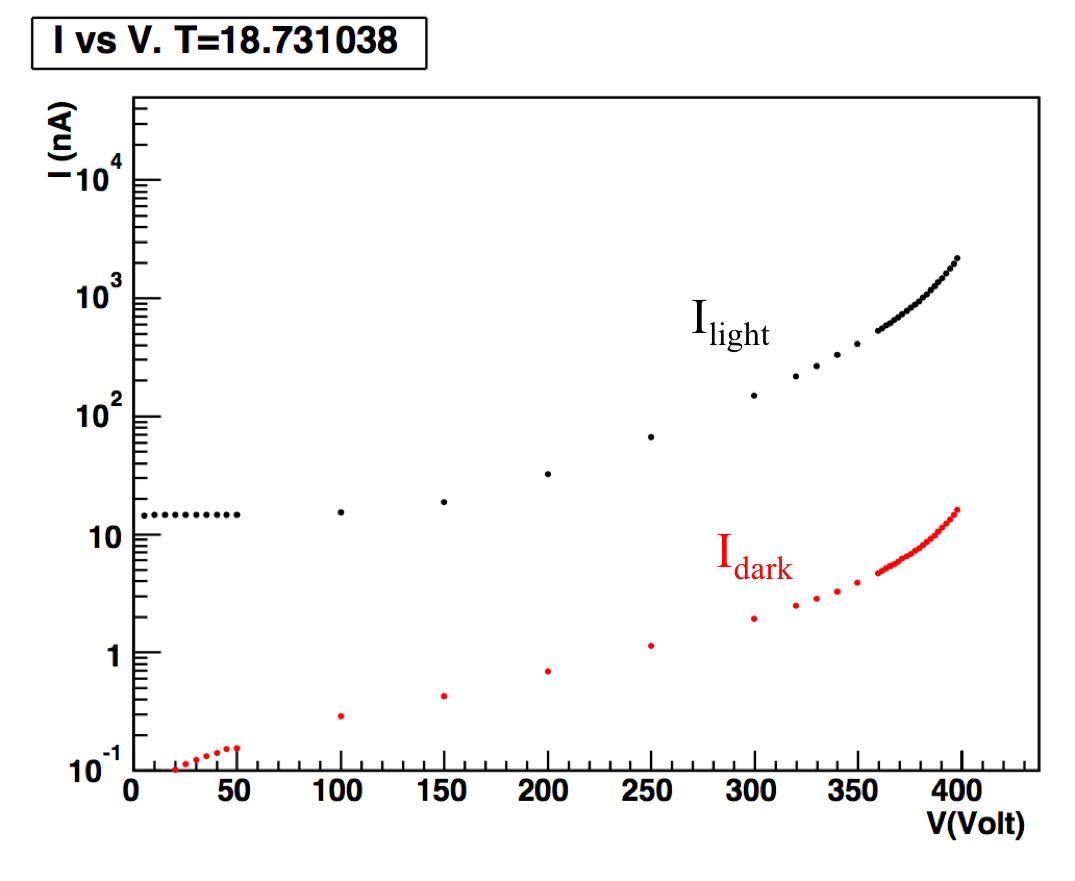
\includegraphics[width=0.5\textwidth]{pics/experiment/apdcurrent.png}
  \caption[APD current draw versus voltage with LED on and off]{The current measured from an individual APD as tested over a range of voltages with both the LED on and off. The measured temperature at the APD for this particular measurement was 18.7~$\degree$C.}
  \label{Figure:apdcurrent}
\end{figure}

The APD gain is calculated by the following relation:

\begin{equation}
	\label{eq:apdgain}
	Gain = \dfrac{I_{light}(V)-I_{dark}(V)}{I_{light}(G=1)-I_{dark}(G=1)} 
\end{equation}
The gain is 1 when the avalanche mechanism is not present. $I_{light}(G=1)$ in Eq.~\eqref{eq:apdgain} is the corresponding light current, and $I_{dark}(G=1)$ is the measured dark current when the gain is 1. Using this relation, the gain can be characterized for all measured dark currents and should have a linear relation. This relationship is shown in Figure~\ref{Figure:apdIvG}.

\begin{figure}[h]
  \centering
      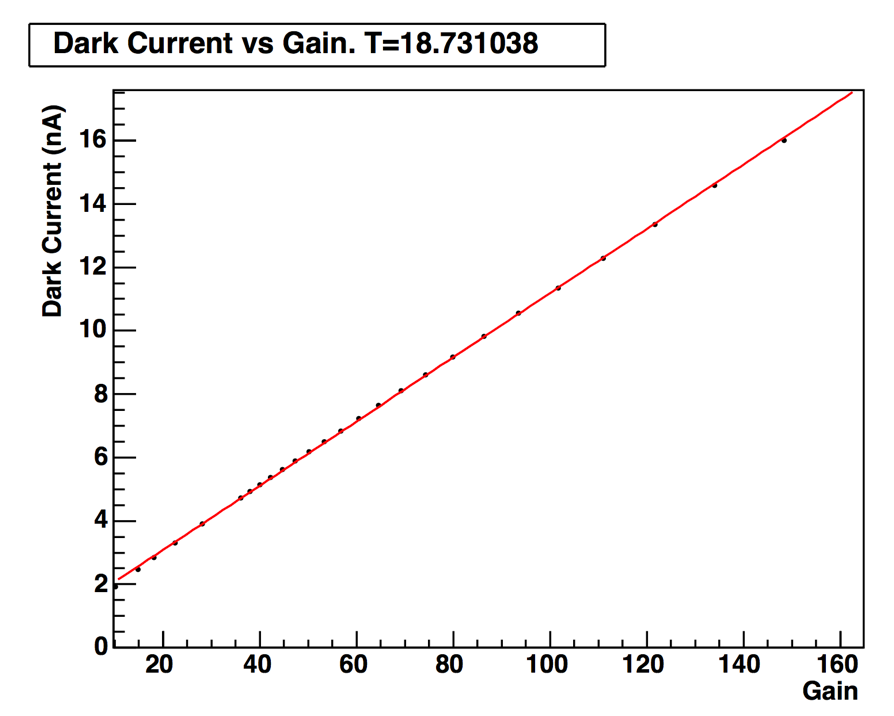
\includegraphics[width=0.5\textwidth]{pics/experiment/apdIvG.png}
  \caption[APD measured dark current as a function of gain]{The dark current measured from an individual APD plotted versus the gain as tested over a range of voltages with both the LED on and off. The measured temperature at the APD for this particular measurement was 18.7$\degree$C.}
  \label{Figure:apdIvG}
\end{figure}

If the relationship between the dark current and the gain is not linear, as shown in Figure~\ref{Figure:apdIvG}, then the APD was re-tested to ensure quality. APDs were placed into 52 common voltage groups ranging from as little as two to a maximum of ten APDs in each group in order to minimize gain variations across the ECal. The grouping temperature was chosen to be 18$\degree$C in order to avoid condensation in the cooling lines of the ECal. The optimal voltage for each APD at 18$\degree$C and a pre-selected gain of 150 can be extrapolated as shown in Figure~\ref{Figure:apdTV}.

\begin{figure}[h]
  \centering
      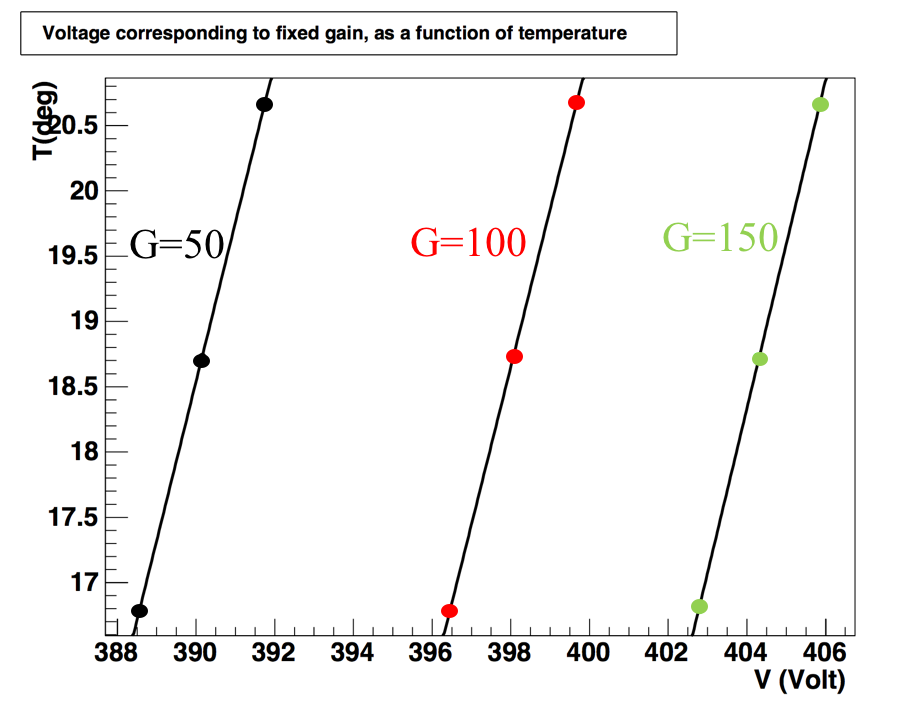
\includegraphics[width=0.5\textwidth]{pics/experiment/apdTV.png}
  \caption[APD fixed gain in terms of voltage and temperature]{The calculated voltages for fixed gains as a function of temperature can be used to group the APDs for common high voltage.}
  \label{Figure:apdTV}
\end{figure}

\section{Trigger}
Events of interest in the HPS experiment are triggered by the ECal. Each channel of the ECal is read out to an FADC250 with 16 channels per board. The FADC250 continuously samples analog signals at a rate of 250~MHz, or every 4~ns, with 12-bit precision. As the data size was small enough, the 2015 and 2016 data was recorded in raw mode such that 100~samples of raw information in a channel are read at the trigger time. This raw mode, called Mode 1, allowed for precise offline pulse fitting of the signals for optimal energy and timing resolution. In the 2015 engineering run, the signals from the ECal were split with $1/3$ of the signal going to TDCs and $2/3$ of the signal going to the FADCs. This was done as a precautionary measure in the event that the new FADCs were unreliable. In the 2016 run, the splitters were removed, allowing for the full signal to go to the FADC due to their proven capabilities. The full readout chain of the ECal trigger is shown in Figure~\ref{Figure:readoutChain}.
\begin{figure}[thb]
  \centering
      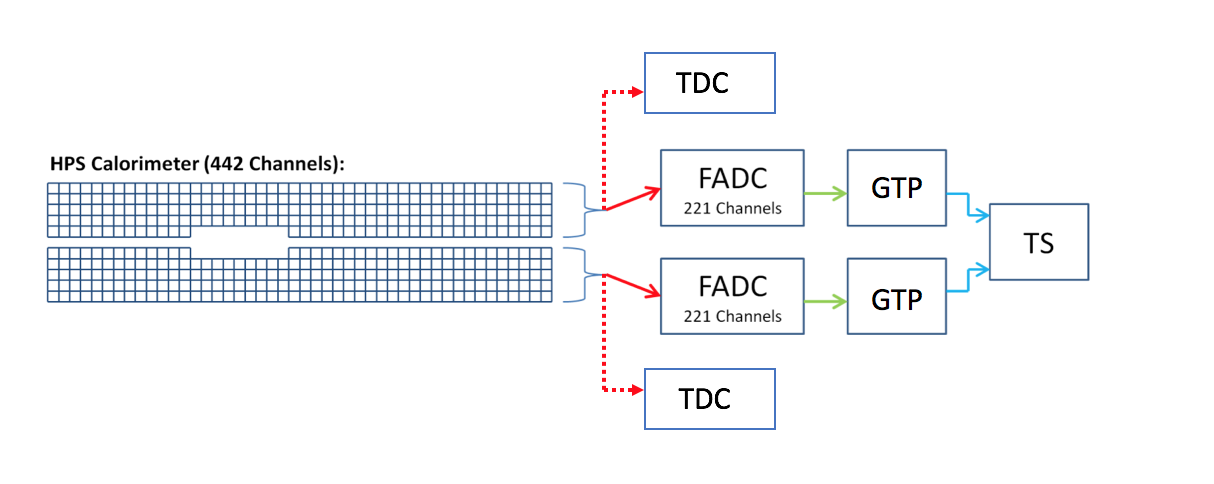
\includegraphics[width=0.75\textwidth]{pics/experiment/readoutChain.png}
  \caption[ECal readout chain]{The Flash ADC continuously samples ECal crystals at 250~MHz. In the 2015 engineering run, signals from the ECal were split with $1/3$ of the signal going to the TDCs and $2/3$ of the signal going to the FADCs. When a signal crosses threshold, the GTP makes $3\times3$ crystal clusters by searching for hits above threshold in adjacent crystals. The trigger supervisor (TS) uses the GTP clusters to make a trigger decision.}
  \label{Figure:readoutChain}
\end{figure}
When a signal crosses a pre-defined threshold, a set number of samples before and after the crossing are summed together to provide a pulse charge value which is converted to energy. The conversion to energy requires access to the individual channel gains and pedestals (as found by cosmic calibrations) which are pre-loaded into the data acquisition (DAQ) system. The energy and time of threshold crossing are sent to the General Trigger Processor (GTP) board every 16~ns  for clustering~\cite{balossino_hps_2016}.\\
\indent The GTP clusterer first identifies the crystal carrying the highest energy (known as the seed hit) in comparison to all surrounding crystals. The immediately neighboring crystals of the seed hit are compared in both energy and time coincidence with respect to the seed crystal in order to create a cluster. The cluster energy is the sum of all of the hits in a cluster. The timing coincidence is typically chosen to be 4~samples to allow for time-walk effects. The cluster information is then passed to the Subsystem Processor (SSP) to make a trigger decision based on various settable trigger cut requirements. \\
\indent The SSP includes several different trigger configurations that can run simultaneously containing different settable cuts and prescale values for ECal modules. The SSP looks for combinations of clusters that pass the configuration requirements and cuts and then sends a trigger to the Trigger Supervisor (TS) board when a cluster or pair of clusters satisfies the trigger requirements. The trigger is then sent to the Trigger Interface (TI) boards in order to trigger readout of all detectors.\\ 
\indent The SSP trigger configurations include two different cluster-pair triggers, two different single-cluster triggers, a random pulser trigger, a cosmic trigger, and an LED trigger of which all except for the cosmic and LED triggers were run during data taking with beam. The first single cluster trigger, Single 1, was optimized for elastically-scattered beam energy electrons off the target. The looser version of the trigger was Single 0. These triggers were useful in selecting events for calibrating the ECal and studying the trigger efficiencies. The cluster-pair trigger is the primary trigger for the HPS experiment and studies all possible combinations of clusters in the ECal for pair selection. It requires one cluster in each half of the ECal. The tuneable cuts used in this trigger are presented in Table~\ref{tab:pairTriggerCuts}~\cite{balossino_hps_2016}. \\
\begin{table}[htb]
\caption{Pair 1 Trigger Cuts}
\label{tab:pairTriggerCuts}
\centering
\begin{tabular}{lc}
\toprule
%\multicolumn{2}{c}{Name} \\
%\cmidrule(r){1-2}
Trigger cut & Cut value \\
\midrule
Time difference & $| t_{top}-t_{bot} | \leq t_{coincidence}$   \\
Cluster energy & $E_{min}<E_{i}<E_{max}$\\
Cluster sum & $E_{sum min}\leq E_1+E_2\leq E_{sum max}$\\
Cluster size & $N_{hits}\geq N_{threshold}$\\
Energy difference & $ E_{2}-E_{1}<E_{difference}$\\
Coplanarity & $ |\arctan\dfrac{x_1}{y_1}-\arctan\dfrac{x_2}{y_2} | \leq \theta_{coplanarity}$\\
Energy-distance & $E_{1}+r_{1}F\geq E_{slope}$ \\ 
\bottomrule
\end{tabular}
\end{table}
The variables $t_i,E_i, N_i, x_i,$ and $y_i$ denote the cluster time, cluster energy, number of hits in the cluster, and coordinates of the cluster, respectively. The subscript, $1$, denotes the cluster with the lowest energy of the pair.  The parameter, $r_1$, is the distance between the center of the lowest energy cluster and the center of the ECal (defined as $r_1=\sqrt{x_1^2+y_1^2}$). The parameters selected for the cuts include the $t_{coincidence}, E_{min}, E_{max}, E_{sum min}, E_{sum max}, N_{threshold}, E_{difference}, \theta_{coplanarity}, r_{1},$ and $E_{slope}$, and are chosen from studying A$^{\prime}$ Monte Carlo in order to optimize the signal acceptance while minimizing the background. The GTP clusters are created prior to track-matching and offline clustering (which includes hits belonging to a cluster beyond those immediately adjacent to the seed hit). For the 2015 data, a GTP cluster conserves roughly 80$\%$ of the fully reconstructed particle energy when the seed hit is not on the edge of the ECal. \\
\indent The time coincidence cut is kept loose enough in the SSP pairs cluster selection to allow for time walk and cabling offsets which are not corrected for until the full pulse is fitted in offline reconstruction. At the GTP stage, the time only corresponds to threshold crossing of the signal. The cluster energy cut selects clusters that are reconstructed by the GTP in the energy range of interest. The minimum hit requirement for clusters was lowered at the start of running due to $A^{\prime}$ Monte Carlo studies indicating that 1 hit clusters were possible and could improve reach without overburdening the trigger. The cluster sum cut most significantly removes accidental pairs containing elastically-scattered beam energy electrons in addition to removing low energy cluster sum events that will not pass thresholds for well-reconstructed events. The energy difference cut removes events that have extremely different cluster energies and do not satisfy $A^{\prime}$-type criteria. \\
\indent The coplanarity cut removes events that are not coplanar including M$\o$ller and wide-angle bremsstrahlung (WAB) backgrounds because the $e^+e^-$ trident events of interest are distributed symmetrically around the beamline. The angle is calculated from the center of the ECal where the beam line passes through to each cluster in the pair relative to the vertical axis. The pairs should be approximately $180\degree$ apart. \\
\indent The energy-distance cut is applied to the lowest-energy cluster of the pair in order to reject events where the cluster is too close to where the electron beam passes through the ECal. Trident kinematics show that these clusters are dominated by bremsstrahlung low energy photons and that there is some reasonable distance of separation with respect to the beamline for these lower energy events. The cut values used in the 2015 Pair 1 trigger are shown in Table~\ref{tab:pairTriggerVals}.\\
\begin{table}[htb]
\caption{Pair 1 trigger cut values for the 2015 engineering run}
\label{tab:pairTriggerVals}
\centering
\begin{tabular}{lc}
\toprule
%\multicolumn{2}{c}{Name} \\
%\cmidrule(r){1-2}
Trigger cut & Cut value \\
\midrule
Time difference & $| t_{top}-t_{bot} | \leq12$ ns   \\
Cluster energy & $54<E<630$ MeV \\
Cluster size & $N_{hits}\geq 1$\\
Energy sum & $180<E_{top}+E_{bot}<860$ MeV\\
Energy difference & $| E_{top}-E_{bot}|<540$ MeV\\
Coplanarity & $\theta_{top}-\theta_{bot}<30\degree $\\
Energy-distance & $E_{1}+(5.5 \textrm{ MeV/mm})r_{1}>600$ MeV\\ 
\bottomrule
\end{tabular}
\end{table}
\indent The pulser trigger generates a constant rate of triggers at 100~Hz regardless of the physics events as measured by the ECal. This makes the pulser an unbiased probe for measuring the backgrounds of the experiment during running with the beam and concurrent with other triggers.\\ 
\indent The cosmic trigger was used without the beam for calibration of the ECal and uses the timing coincidence between two scintillators, placed below and external to the ECal, in order to trigger readout of all ECal channels for offline reconstruction of the cosmic event. The timing coincidence of the scintillators placed in line and below the ECal was chosen to be 40~ns where the leading edge of the scintillator signal in the FADC pulse crosses 60~ADC samples. Once the timing and threshold conditions are met, all modules in the ECal were readout in Mode 1 format. 
